\documentclass[answers]{exam}
\usepackage{../../mypackages}
\usepackage{../../macros}

\setlength{\parindent}{0pt}

\SolutionEmphasis{\color{blue}}
\renewcommand{\solutiontitle}{\noindent}

\title{DST N°3 - Photographie + Lumière}
\author{N. Bancel}
\date{19 Mars 2025}

\begin{document}

\textbf{Collège Lycée Suger}
\hfill
\textbf{Physique-Chimie} \\

\textbf{Année 2024-2025 - 3ème trimestre}
\hfill
\textbf{1ère STD2A} \par

{\let\newpage\relax\maketitle}


\begin{center}
  \textbf{\textcolor{blue}{Durée du devoir : 2 heures}} \par
  \vspace{1em}
  \textbf{\textcolor{red}{La calculatrice EST autorisée. Total des points : 20 points}} \par
  \vspace{1em}
\end{center}

\begin{tcolorbox}[colback=gray!10!white, colframe=gray, title=Note importante]
  \itshape{Toutes les réponses doivent être justifiées.
  La qualité et la précision de la rédaction seront prises en compte dans la notation des copies.
  Il est permis d'admettre le résultat de certaines questions pour ne pas rester bloqué, en prenant soin d'indiquer sur la copie les résultats admis. \par
  }
\end{tcolorbox}

\section*{Exercice 2 - Lumière (5 points)}

\textit{Extrait du BAC 2018 - Polynésie}

\begin{figure}[H]
  \centering
  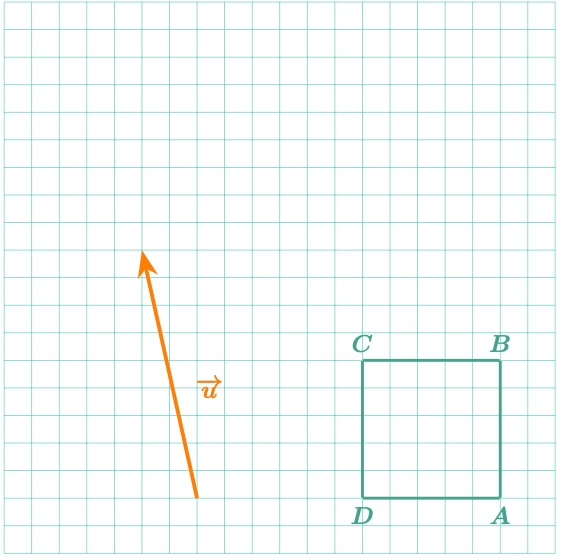
\includegraphics[width=0.7\textwidth]{img/dst_03_01.jpg}
  \caption{Verre du musée}
  \label{fig:bioluminescence}
\end{figure}

\begin{questions}
  \question[0.5] Citer le constituant principal d'un verre minéral.
  \question[0.5] Préciser à quel type d'ondes appartiennent les rayonnements ultraviolets, visibles et infrarouges cités dans le document 4.
  \question[4] On considère un rayonnement de longueur d'onde dans le vide $\lambda$ égale à 900 nm.
  \begin{parts}
      \part[1] Indiquer à quel domaine appartient ce rayonnement : ultraviolet, lumière visible, infrarouge, en expliquant ce choix.
      \part[1] Déterminer la fréquence de ce rayonnement.
      \part[2] Déterminer l'énergie d'un photon associé à ce rayonnement.
  \end{parts}
\end{questions}

\section*{Exercice 3 - Restauration des vitraux (3.5 points)}

  \textit{Extrait du BAC 2018 - Métropoloe}

\begin{figure}[H]
  \centering
  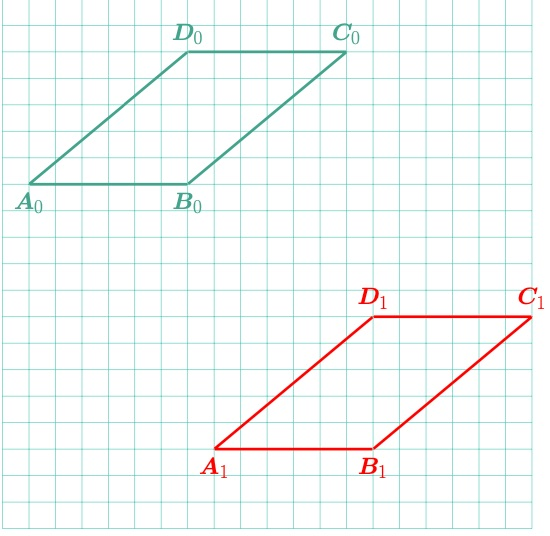
\includegraphics[width=0.7\textwidth]{img/dst_03_02.jpg}
  \caption{Nettoyage des dépôts blancs}
\end{figure}

\begin{figure}[H]
  \centering
  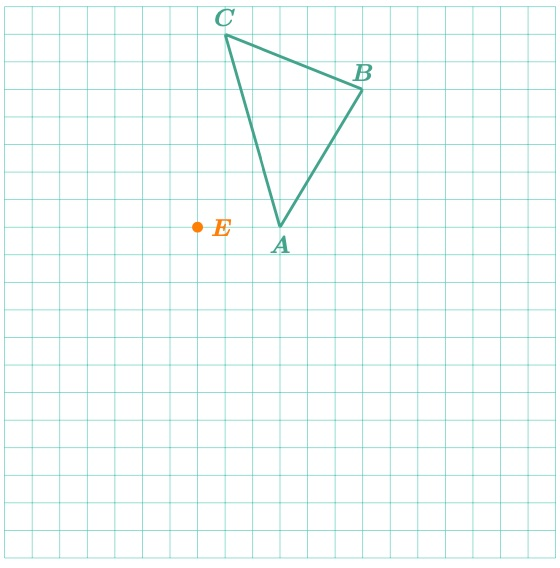
\includegraphics[width=0.7\textwidth]{img/dst_03_03.jpg}
\end{figure}


\begin{questions}
  \question[0.5] Déterminer la nature des deux rayonnements utilisés pour l'analyse spectroscopique des dépôts blancs.
  \question[1] Préciser, sans calcul, lequel des deux rayonnements est le plus énergétique.
  \question[1] Déterminer les longueurs d'onde minimale et maximale des rayonnements infrarouges
  \question[1] Déterminer les informations révélées par l'analyse du dépôt blanc.
\end{questions}

\end{document}

